\documentclass[twocolumn,a4j]{jsarticle}
\setlength{\topmargin}{-20.4cm}
\setlength{\oddsidemargin}{-10.4mm}
\setlength{\evensidemargin}{-10.4mm}
\setlength{\textwidth}{18cm}
\setlength{\textheight}{26cm}

\usepackage[top=15truemm,bottom=20truemm,left=20truemm,right=20truemm]{geometry}
\usepackage[latin1]{inputenc}
\usepackage{amsmath}
\usepackage{amsfonts}
\usepackage{amssymb}
\usepackage[dvipdfmx]{graphicx}
\usepackage[hang,small,bf]{caption}
\usepackage[subrefformat=parens]{subcaption}
\usepackage[dvipdfmx]{color}
\usepackage{listings}
\usepackage{listings,jvlisting}
\usepackage{geometry}
\usepackage{framed}
\usepackage{color}
\usepackage[dvipdfmx]{hyperref}
\usepackage{ascmac}
\usepackage{enumerate}
\usepackage{tabularx}
\usepackage{cancel}
\usepackage{scalefnt}
\usepackage{overcite}
\usepackage{otf}
\usepackage{multicol}
\usepackage[geometry]{ifsym}

\renewcommand{\figurename}{Fig.}
\renewcommand{\tablename}{Table }

\hypersetup{%
    hidelinks %リンクの色消し
}

\lstset{
basicstyle={\ttfamily},
identifierstyle={\small},
commentstyle={\smallitshape},
keywordstyle={\small\bfseries},
ndkeywordstyle={\small},
stringstyle={\small\ttfamily},
frame={tb},
breaklines=true,
columns=[l]{fullflexible},
xrightmargin=0zw,
xleftmargin=3zw,
numberstyle={\scriptsize},
stepnumber=1,
numbersep=1zw,
lineskip=-0.5ex
}

% キャプション後ろのダブルコロンを消す
\makeatletter
\long\def\@makecaption#1#2{%
  \vskip\abovecaptionskip
  \iftdir\sbox\@tempboxa{#1\hskip1zw#2}%
    \else\sbox\@tempboxa{#1 #2}%
  \fi
  \ifdim \wd\@tempboxa >\hsize
    \iftdir #1\hskip1zw#2\relax\par
      \else #1 #2\relax\par\fi
  \else
    \global \@minipagefalse
    \hbox to\hsize{\hfil\box\@tempboxa\hfil}%
  \fi
  \vskip\belowcaptionskip}
\makeatother


\makeatletter
\def\@maketitle
{
\begin{center}
{\LARGE \@title \par}
\end{center}
\begin{flushright}
{\large \@date}\\
{\large 京都工芸繊維大学 大学院 機械設計学専攻 計測システム工学研究室}\\
{\large M2 \@author}
\end{flushright}
\par\vskip 1.5em
}
\makeatother

\author{来代 勝胤 / KITADAI Masatsugu}
\title{令和5年度 9月度 共同研究報告書}
\date{2023/09/29}

\begin{document}
\columnseprule=0.1mm
\maketitle

\section*{報告内容}
\begin{enumerate}[1.]
	\item 概要:二次流れの解析手法
	\item 粒子クラスタの取得
	\item マッチング方法
	\item 流れの解析結果
	\item 11月の予定
\end{enumerate}

\section*{進捗報告}
今月は,先月に引き続き局所的な流れに対応した二次流れ解析の実現に向けて
解析手法の検討を行った.そこで,同一粒子の粒子像から構成される粒子クラスタを取得し,
その情報を用いて粒子追跡のアルゴリズムを作成した.
その結果,これまで計測できていなかった
車両モデルの流れ場について,
タイヤの回転の有無の効果と先行研究に示される流れ構造を確認することができた.

\section{概要:二次流れの解析手法}
\begin{figure}[htbp]
	\centering
	\includegraphics[keepaspectratio, width=82mm]{../images/method.png}
	\caption{PTV method for secondary flow analysis}
\end{figure}

\begin{figure}[htbp]
	\centering
	\includegraphics[keepaspectratio, width=82mm]{../images/experiment.png}
	\caption{Experiment setup}
\end{figure}

\section{粒子位置の特定}

\begin{figure}[htbp]
	\centering
	\includegraphics[keepaspectratio, width=82mm]{../images/closs-correlation_for_particle.png}
	\caption{Cross-correlation for particle image}
	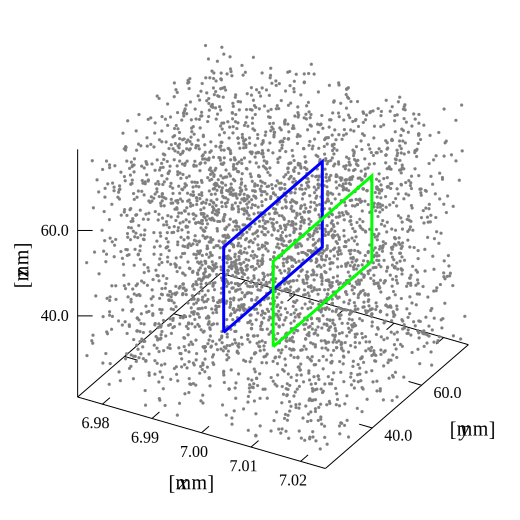
\includegraphics[keepaspectratio, width=82mm]{../images/particle_position.png}
	\caption{Particle position for green image}
\end{figure}

\section{粒子クラスタの取得}

\begin{figure}[htbp]
	\centering
	\includegraphics[keepaspectratio, width=50mm]{../images/how_to_get_cluster.png}
	\caption{PTV for clustering}
\end{figure}

\begin{figure}[htbp]
	\centering
	\includegraphics[keepaspectratio, width=82mm]{../images/clustering_for_blue_image.png}
	\caption{Clustering for blue image}
\end{figure}

\section{クラスタマッチング}

\section{流れの解析結果}

\subsection{車両モデル}
\begin{figure}[htbp]
	\centering
	\includegraphics[keepaspectratio, width=80mm]{../images/delta_wing_model.png}
	\caption{PTV Measurement : Vehicle model without tire rotation}
\end{figure}


\subsection{三角翼後流}
\begin{figure}[htbp]
	\centering
	\includegraphics[keepaspectratio, width=82mm]{../images/delta_wing.png}
	\caption{PTV :Wake of delta wing}
\end{figure}

\subsection{車両モデル}
\begin{figure}[htbp]
	\centering
	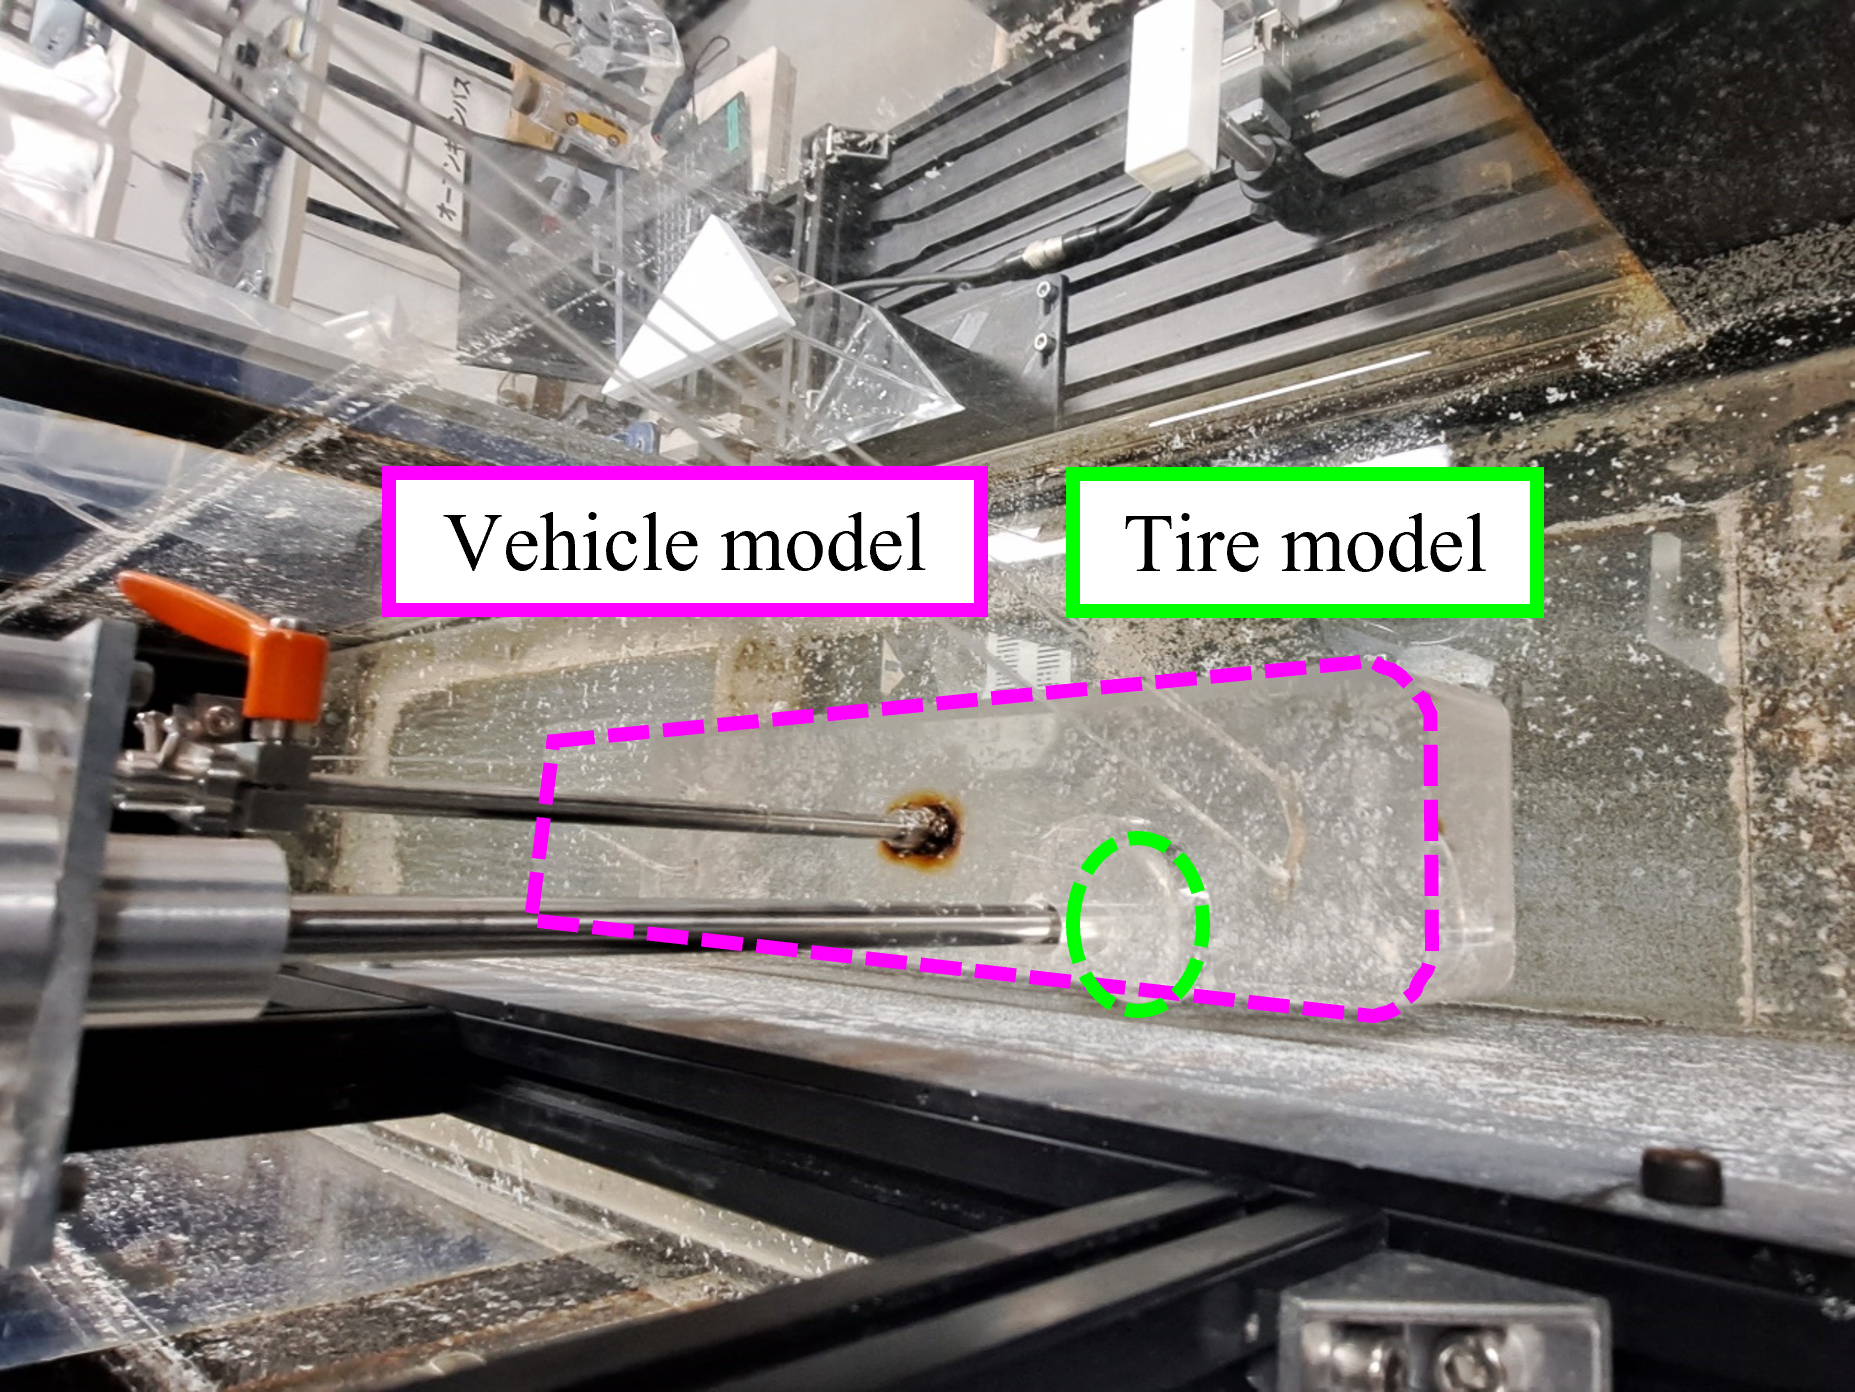
\includegraphics[keepaspectratio, width=80mm]{../images/vehicle_model.png}
	\caption{PTV : Vehicle model without tire rotation}
\end{figure}


\subsection{タイヤ回転:無}
\begin{figure}[htbp]
	\centering
	\includegraphics[keepaspectratio, width=82mm]{../images/vehicle_stop.png}
	\caption{PTV : Vehicle model without tire rotation}
\end{figure}


\subsection{タイヤ回転:有}
\begin{figure}[htbp]
	\centering
	\includegraphics[keepaspectratio, width=82mm]{../images/vehicle_rolling.png}
	\caption{PTV Measurement :Vehicle model with tire rotation}
\end{figure}



\section{11月の予定}
\begin{itemize}
	\item 車両モデルの計測
	\item 数値シミュレーションによる性能評価
\end{itemize}


\end{document}